\begin{pages}
    \begin{Rightside}
    \selectlanguage{greek}
        \beginnumbering
        \pstart[
        			\chapter{Ἡ κρίσις ἡ ἐσχάτη}
        			\markboth{The Last Judgement}
				]
		\renewcommand{\LettrineFontHook}{\PHtitl}
		\lettrine[lines=3]{Κ}{αὶ} εἶδον ἄγγελον καταβαίνοντα ἐκ τοῦ οὐρανοῦ, ἔχοντα τὴν κλεῖν τῆς ἀβύσσου καὶ ἅλυσιν μεγάλην ἐπὶ τὴν χεῖρα αὐτοῦ. καὶ ἐκράτησεν τὸν δράκοντα, ὁ ὄφις ὁ ἀρχαῖος, ὅς ἐστιν Διάβολος καὶ Ὁ Σατανᾶς, καὶ ἔδησεν αὐτὸν χίλια ἔτη, καὶ ἔβαλεν αὐτὸν εἰς τὴν ἄβυσσον, καὶ ἔκλεισεν καὶ ἐσφράγισεν ἐπάνω αὐτοῦ, ἵνα μὴ πλανήσῃ ἔτι τὰ ἔθνη, ἄχρι τελεσθῇ τὰ χίλια ἔτη· μετὰ ταῦτα δεῖ λυθῆναι αὐτὸν μικρὸν χρόνον. 
		\pend
		\pstart
		Καὶ εἶδον θρόνους, καὶ ἐκάθισαν ἐπ’ αὐτούς, καὶ κρίμα ἐδόθη αὐτοῖς, καὶ τὰς ψυχὰς τῶν πεπελεκισμένων διὰ τὴν μαρτυρίαν Ἰησοῦ καὶ διὰ τὸν λόγον τοῦ Θεοῦ, καὶ οἵτινες οὐ προσεκύνησαν τὸ θηρίον οὐδὲ τὴν εἰκόνα αὐτοῦ καὶ οὐκ ἔλαβον τὸ χάραγμα ἐπὶ τὸ μέτωπον καὶ ἐπὶ τὴν χεῖρα αὐτῶν· καὶ ἔζησαν καὶ ἐβασίλευσαν μετὰ τοῦ Χριστοῦ χίλια ἔτη. οἱ λοιποὶ τῶν νεκρῶν οὐκ ἔζησαν ἄχρι τελεσθῇ τὰ χίλια ἔτη. αὕτη ἡ ἀνάστασις ἡ πρώτη. μακάριος καὶ ἅγιος ὁ ἔχων μέρος ἐν τῇ ἀναστάσει τῇ πρώτῃ· ἐπὶ τούτων ὁ δεύτερος θάνατος οὐκ ἔχει ἐξουσίαν, ἀλλ’ ἔσονται ἱερεῖς τοῦ Θεοῦ καὶ τοῦ Χριστοῦ, καὶ βασιλεύσουσιν μετ’ αὐτοῦ τὰ χίλια ἔτη. 
		\pend
		\pstart
		Καὶ ὅταν τελεσθῇ τὰ χίλια ἔτη, λυθήσεται ὁ Σατανᾶς ἐκ τῆς φυλακῆς αὐτοῦ, καὶ ἐξελεύσεται πλανῆσαι τὰ ἔθνη τὰ ἐν ταῖς τέσσαρσιν γωνίαις τῆς γῆς, τὸν Γὼγ καὶ Μαγώγ, συναγαγεῖν αὐτοὺς εἰς τὸν πόλεμον, ὧν ὁ ἀριθμὸς αὐτῶν ὡς ἡ ἄμμος τῆς θαλάσσης. καὶ ἀνέβησαν ἐπὶ τὸ πλάτος τῆς γῆς, καὶ ἐκύκλευσαν τὴν παρεμβολὴν τῶν ἁγίων καὶ τὴν πόλιν τὴν ἠγαπημένην· καὶ κατέβη πῦρ ἐκ τοῦ οὐρανοῦ καὶ κατέφαγεν αὐτούς· καὶ ὁ διάβολος ὁ πλανῶν αὐτοὺς ἐβλήθη εἰς τὴν λίμνην τοῦ πυρὸς καὶ θείου, ὅπου καὶ τὸ θηρίον καὶ ὁ ψευδοπροφήτης, καὶ βασανισθήσονται ἡμέρας καὶ νυκτὸς εἰς τοὺς αἰῶνας τῶν αἰώνων. 
		\pend
		\pstart
		Καὶ εἶδον θρόνον μέγαν λευκὸν καὶ τὸν καθήμενον ἐπ’ αὐτόν οὗ ἀπὸ τοῦ προσώπου ἔφυγεν ἡ γῆ καὶ ὁ οὐρανός, καὶ τόπος οὐχ εὑρέθη αὐτοῖς. καὶ εἶδον τοὺς νεκρούς, τοὺς μεγάλους καὶ τοὺς μικρούς, ἑστῶτας ἐνώπιον τοῦ θρόνου, καὶ βιβλία ἠνοίχθησαν· καὶ ἄλλο βιβλίον ἠνοίχθη, ὅ ἐστιν τῆς ζωῆς· καὶ ἐκρίθησαν οἱ νεκροὶ ἐκ τῶν γεγραμμένων ἐν τοῖς βιβλίοις κατὰ τὰ ἔργα αὐτῶν. καὶ ἔδωκεν ἡ θάλασσα τοὺς νεκροὺς τοὺς ἐν αὐτῇ, καὶ ὁ θάνατος καὶ ὁ Ἅιδης ἔδωκαν τοὺς νεκροὺς τοὺς ἐν αὐτοῖς, καὶ ἐκρίθησαν ἕκαστος κατὰ τὰ ἔργα αὐτῶν. καὶ ὁ θάνατος καὶ ὁ Ἅιδης ἐβλήθησαν εἰς τὴν λίμνην τοῦ πυρός. οὗτος ὁ θάνατος ὁ δεύτερός ἐστιν, ἡ λίμνη τοῦ πυρός. καὶ εἴ τις οὐχ εὑρέθη ἐν τῇ βίβλῳ τῆς ζωῆς γεγραμμένος, ἐβλήθη εἰς τὴν λίμνην τοῦ πυρός.
		\pend
        \endnumbering
    \end{Rightside}
    \begin{Leftside}
        \beginnumbering
        \pstart[
        			\chapter{The Last Judgement}
				]		
		\renewcommand{\LettrineFontHook}{\Zallmanfamily}
		\lettrine[lines=3]{A}{nd} I saw an angel coming down from Heaven, having the keys of the abyss and a great chain in his hand. And he seized the dragon — the ancient serpent — who is (the) Devil and (the) Satan and he bound him for a thousand years. And he threw him into the abyss and he locked and sealed (the opening) above him so that he may no longer deceive the nations until the thousand years have passed (lit. are finished). And thereafter he must be loosened for a little while. 
		\pend
		\pstart
		And I saw thrones and they (the apostles / saints) sat upon them and (the authority to pass) a judgement was given to them; and their souls were beheaded because of the witness of Jesus and because of the word of God and whoever did not worship the beast or its idol (and whoever did) not take the mark upon his forehead and upon his hand. And they lived and reigned with Christ for a thousand years. The remaining of the dead did not live until the thousand years have passed (lit. have finished). This is the first resurrection. Blessed and holy is he who has a part in the first resurrection, (for) the second death has no authority over them but they will (instead) be priests of God and Christ; and they will reign with Him for a thousand years. 
		\pend
		\pstart
		And when the thousand years have passed (lit. are finished), Satan will be freed from his prison and he will come out to deceive the nations, (namely) those in the four corners of the Earth — (the) Gog and Magog — (and he does this in order) to gather (and prepare) them (to go) into battle; (and) their number is as (large) as the (amount of grains of) sand of the sea. And they went up onto the breadth of the Earth (land) (i. e. they covered its entire breadth) and they surrounded the camp of the holy men and the (be)loved city. And fire descended out of Heaven and ate them (up). And the Devil — the one who deceived them (their deceiver) — was thrown into the lake of fire and brimstone (sulphur); (the same place) where even the beast and the false prophet will be tormented day and night into the eternity of eternities (forever).
		\pend
		\pstart
		And I saw a great, white throne and (I saw) him who sits upon it, from whose face the Earth and the Heaven fled — and no place was found for them. And I saw the dead — the great and the small — standing before the throne; and books were opened. And another book was opened, (the one) which is (the book) of life. And the dead were judged according to their deeds (as they were recorded in) from the writings of the books. And the sea gave (up) the dead (that were) within it, and Death and Hades gave (up) the dead (which were) within them; and they were each judged according to their deeds. And Death and Hades were thrown into the lake of fire. This is the second death — the lake of fire. And if someone (’s name) was not found written in the book of life, he was thrown into the lake of fire. 
		\pend
        \endnumbering
    \end{Leftside}

\end{pages} 
\Pages

\clearpage
\thispagestyle{empty}
\null\vfill
\settowidth\longest{\huge\itshape […] and when I turned around I saw}
\begin{center}
\parbox{\longest}{%
  \raggedright{\huge\itshape%
    ``And the dead were judged according to their deeds […]'' \par\bigskip
  }
  \raggedleft\Large\MakeUppercase{``The Last Judgement'' — John Martin, 1853}\par%
}
\vfill\vfill
\clearpage\newpage
\end{center}
\newpage
\thispagestyle{empty}
\begin{center}
	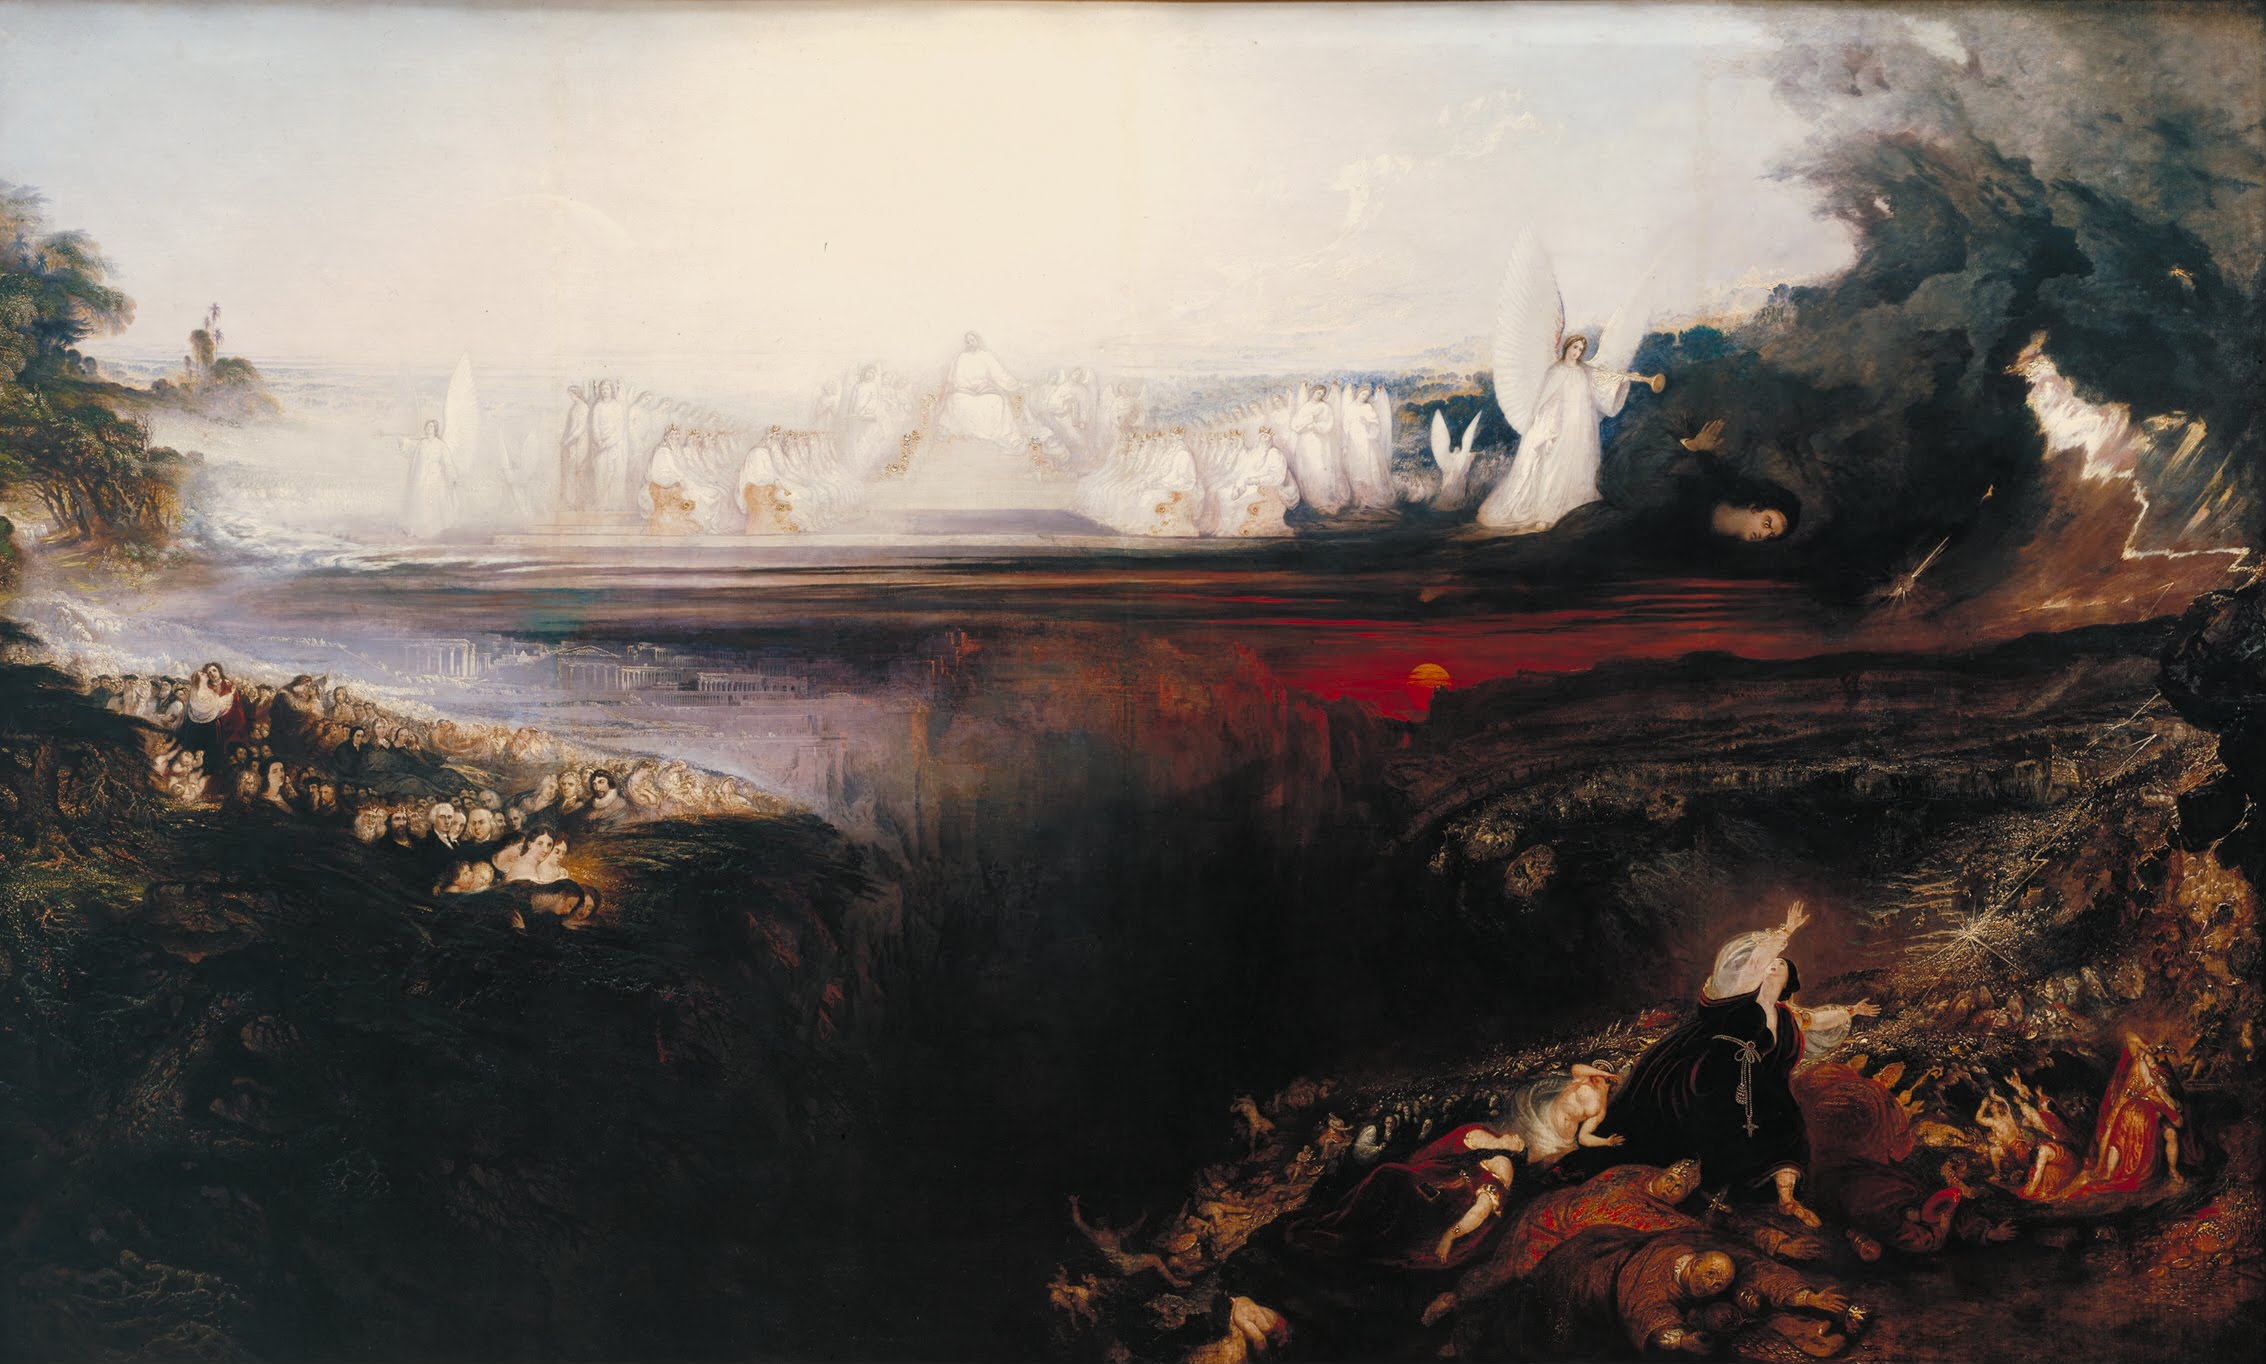
\includegraphics[angle=90, width=0.85\textwidth]{images/illustrations/johnmartinjudgement}
\end{center}